\documentclass{article}%
\usepackage[T1]{fontenc}%
\usepackage[utf8]{inputenc}%
\usepackage{lmodern}%
\usepackage{textcomp}%
\usepackage{lastpage}%
\usepackage[head=40pt,margin=0.5in,bottom=0.6in]{geometry}%
\usepackage{graphicx}%
%
\title{\textbf{Trabajadores protestan en Guayana por mejoras salariales}}%
\author{El Nacional Web}%
\date{01/10/2018}%
%
\begin{document}%
\normalsize%
\maketitle%
\textbf{URL: }%
http://www.el{-}nacional.com/noticias/protestas/trabajadores{-}protestan{-}guayana{-}por{-}mejoras{-}salariales\_253815\newline%
%
\textbf{Periodico: }%
EN, %
ID: %
253815, %
Seccion: %
Protestas\newline%
%
\textbf{Palabras Claves: }%
Protestas, Bolívar, Sociedad\newline%
%
\textbf{Derecho: }%
2.3%
, Otros Derechos: %
NO\_TIENE%
, Sub Derechos: %
2.3.4%
\newline%
%
\textbf{EP: }%
SI\newline%
\newline%
%
\textbf{\textit{Un grupo de personas cerró una avenida de la entidad para rechazar los tabuladores del salario}}%
\newline%
\newline%
%
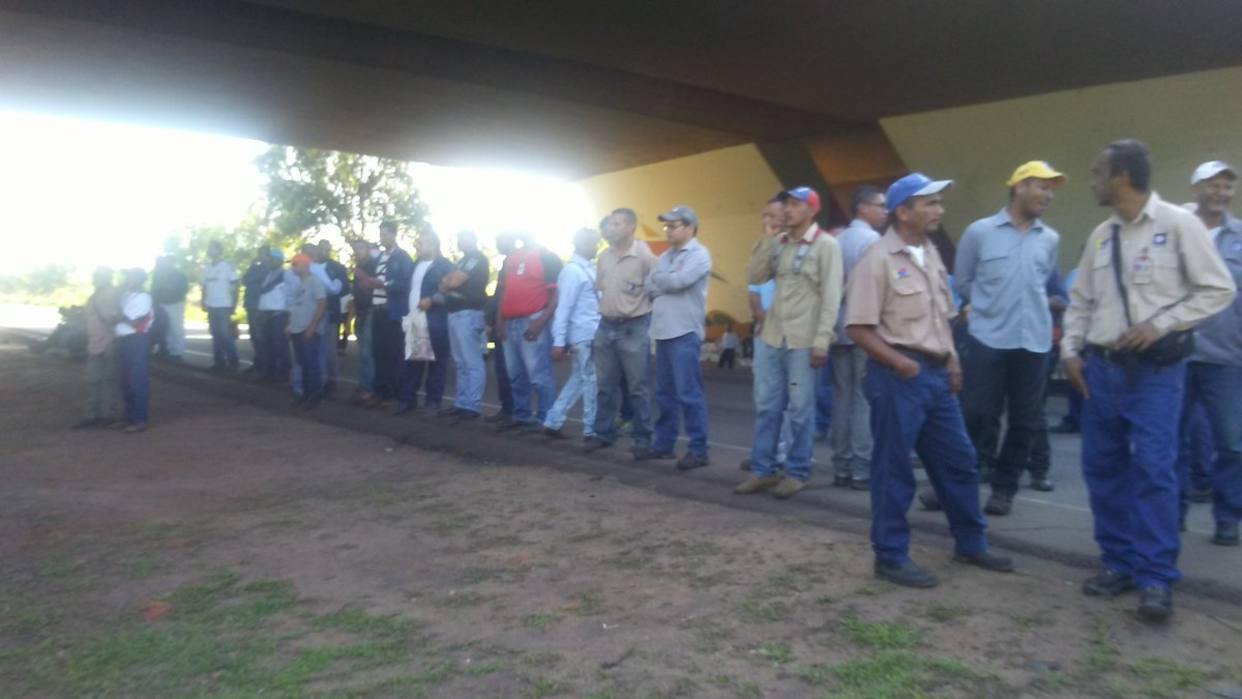
\includegraphics[width=300px]{181.jpg}%
\newline%
%
Un grupo de trabajadores protesta la mañana de este lunes en la avenida Guayana, ubicada en el estado Bolívar, para rechazar el tabulador salarial.%
\newline%
%
La periodista Pableysa Ostos informó que las personas se encuentran a la altura del elevado de CVG Carbonara.%
\newline%
%
En imágenes difundidas vía Twitter se puede observar que los trabajadores se encuentran en el lugar mientras obstaculizan el paso de los vehículos.%
\newline%
%
\end{document}